%% Journal of Open Research Software Latex template -- Created By Stephen Bonner and John Brennan, Durham Universtiy, UK.

\documentclass{jors}

%% Set the header information
\pagestyle{fancy}
\definecolor{mygray}{gray}{0.6}
\renewcommand\headrule{}
\rhead{\footnotesize 3}

\usepackage{biblatex}
\usepackage{hyperref}
\bibliography{paper}

\usepackage{graphicx}
\usepackage{hyperref}



\begin{document}

\newcommand\githublink[1]{\href{https://github.com/#1/}{\texttt{\textbf{@#1}}}}
%% {\bf Software paper for submission to the Journal of Open Research Software} \\

%% To complete this template, please replace the blue text with your own. The paper has three main sections: (1) Overview; (2) Availability; (3) Reuse potential. \\

%% Please submit the completed paper to: editor.jors@ubiquitypress.com

%% \rule{\textwidth}{1pt}

\section*{(1) Overview}

\vspace{0.5cm}

\section*{Title}

PFHub: The Phase-Field Community Hub

\section*{Paper Authors}

1. Wheeler, Daniel; (corresponding author) A\\
2. Keller, Trevor; A\\
3. DeWitt, Stephen J.; E\\
4. Jokisaari, Andrea M.; D\\
5. Schwen, Daniel; D\\
6. Guyer, Jonathan E.; A\\
7. Aagesen, Larry; D\\
8. Heinonen, Olle G.; B\\
9. Voorhees, Peter W.; C\\
10. Warren, James A.; G

\section*{Paper Author Roles and Affiliations}

A. Materials Science and Engineering Division, \\
Material Measurement Laboratory, \\
National Institute of Standards and Technology,\\
Gaithersburg, MD 20899 USA

B. Argonne National Laboratory, \\
Lemont, IL 60439 USA

C. Department of Materials Science and Engineering, \\
Northwestern University, \\
Evanston, IL 60208 USA

D. Fuel Modeling and Simulation Department, \\
Idaho National Laboratory, \\
Idaho Falls, ID 83415 USA

E. Materials Science and Engineering Department, \\
University of Michigan, \\
Ann Arbor, MI 48109 USA

F. Materials Science and Engineering Department, \\
University of Michigan, \\
Ann Arbor, MI 48109 USA

G. Material Measurement Laboratory Office, \\
Material Measurement Laboratory, \\
National Institute of Standards and Technology,\\
Gaithersburg, MD 20899 USA

\section*{Abstract}

Scientific research communities often require an online portal to
summarize a shared challenge, collect attempts at a solution, and
present a quantitative comparison of past attempts in a compelling
way. An exemplar of such a portal is $\mu$MAG~\cite{mumag}. The
reusable PFHub framework leverages existing online services to build a
static portal website that is considerably easier to deploy and
maintain without sacrificing content or scope. The first deployment of
the PFHub framework supports phase-field practitioners and code
developers participating in an effort to improve quality assurance for
phase-field codes.

\section*{Keywords}

phase-field; materials-science; jekyll-website; reproducible-science

\section*{Introduction}

The phase-field method (PFM) describes material interfaces at the
mesoscopic scale between atomic scale models and macroscale models.
The PFM is well established and there are an assortment of code
frameworks (\emph{e.g} Moose~\cite{moose},
PRISMS-PF~\cite{prisms-pf}, FiPy~\cite{fipy}, MMSP~\cite{mmsp})
available for solving the wide variety of phenomena associated with
phase-field (\emph{e.g.} dendritic growth, spinodal decomposition,
grain growth). However, phase-field research groups often develop
codes in isolation and do not publish the code bases or do not support
or distribute the code bases to the wider community. PFHub is a
community effort spearheaded by the Center for Hierarchical Materials
Design at Northwestern University and the National Institute of
Standards and Technology to support the development of phase-field
codes. The goal of PFHub is to improve cross-collaboration between
phase-field code developers and practitioners by providing a
standardized set of benchmark problems~\cite{bm1, bm2} along with a
web framework for uploading and comparing benchmark results from
different codes.

\section*{Implementation and architecture}

The PFHub website provides a facility for uploading, displaying and
comparing results from the benchmark problems. The website uses the
Jekyll static website generator~\cite{jekyll} along with automated
frontend processing to eliminate the need for content management
systems~\cite{cmsfree}, which are generally costly to maintain
especially for small scientific communities with limited funding and
manpower.

The workflow for uploading benchmark results relies on third party
tools using the following steps, illustrated in
Figure~\ref{fig:pfhub_website}.

\begin{itemize}
  \item The users are first required to archive simulation outputs at
    an archival resource (\emph{e.g.} Figshare) configured with
    permissive cross-origin resource sharing (CORS).
  \item The metadata summarizing each simulation is entered into a
    form on the website, including relevant details such as memory
    usage, run time and links to the data archived in the first step.
  \item Upon submission, the Staticman app~\cite{staticman} submits
    the entered metadata as a GitHub pull request to the PFHub GitHub
    repository.  The metadata is stored in a YAML file with a unique
    path in the repository.
  \item Travis CI~\cite{travis} performs linting on the submission and
    then launches a new version of the website using
    Surge~\cite{surge}. The PFHub admins can then examine the new
    submission and further changes can be made if necessary.
  \item Once review has been completed to the satisfaction of both the
    uploading scientist and the website maintainers, the pull request
    is merged and served to the World Wide Web using a hosting service
    compatible with GitHub Pages.
\end{itemize}

A combination of Jekyll templates and Coffeescript are used to access
and download the data links in the submitted YAML files and then
display the data in interactive figures on the website. The
combination of a central repository on GitHub for website source code
and metadata with distributed data records on third-party archives
avoids the complexity and administrative overhead of maintaining a
live database and associated backend app. The PFHub infrastructure
provides a template for other small scientific communities to host
custom content and integrate data from members of their community.

\begin{figure}
  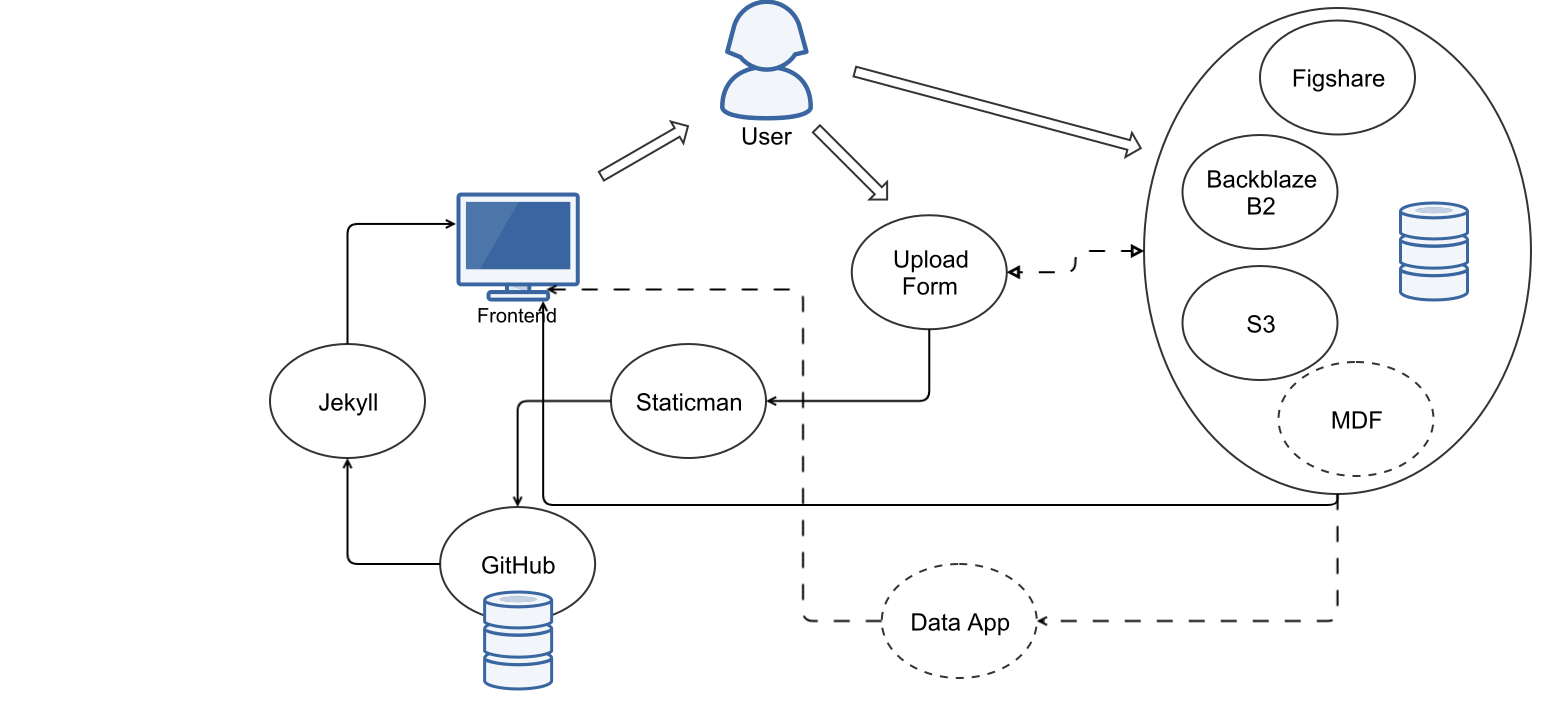
\includegraphics[width=4in]{pfhub_website.png}
  \caption{Schematic overview of the PFHub framework for building
    scientific research portals, simply.}
  \centering
  \label{fig:pfhub_website}
\end{figure}

\section*{Quality control}

The framework has a fully automated test recipe deployed on Travis CI
with an environment built using the Nix Package
Manager~\cite{nix}. The environment is pinned to a specific version of
the Nixpkgs repository ensuring fully reproducible build and test
phases as well as ensuring that the development and automated testing
environments are identical. The full test recipe is outlined in a
\texttt{.travis.yml} file stored in the repository~\cite{travisyml}
and consists of the following steps.

\begin{itemize}
  \item Build the Nix environment from a cached storage reducing the
    build time.
  \item Run automated tests on Jupyter Notebooks using
    NBval~\cite{nbval} and Py.test~\cite{pytest}.
  \item Lint and test front-end Coffeescript using appropriate tools.
  \item Display a temporary version of the website using
    Surge~\cite{surge} for visual review.
\end{itemize}

\section*{(2) Availability}
\vspace{0.5cm}
\section*{Operating system}

The PFHub framework can be deployed on any platform supporting Nix,
which includes all contemporary Linux and Mac OS X platforms. However,
since the framework is built with Jekyll and automated front-end
processing it can be deployed on GitHub's Pages infrastructure.

\section*{Programming language}

PFHub is currently built and tested using the programming language and
versions outlined in Table~\ref{tab:versions}.

\begin{table}[h!]
  \centering
  \caption{PFHub programming languages and corresponding supported
    versions.}
  \begin{tabular}{|l|l|}
    \hline
    Language         & Version \\
    \hline
    HTML             & 5       \\
    Jupyter Notebook & 5.4.0   \\
    JavaScript       & 5       \\
    Nix              & 2.1.3   \\
    CoffeeScript     & 1.12.7  \\
    CSS              & 4       \\
    \hline
  \end{tabular}
  \label{tab:versions}
\end{table}


\section*{Additional system requirements}

There are no additional system requirements.

\section*{Dependencies}

The entire environment can be built using the Nix Package Manager so
the only required dependency is a functional Nix installation. The
full set of dependencies are extensive and fully outlined in the Nix
recipe stored in the repository~\cite{nix-recipe}.

\section*{List of contributors}

1. Wheeler, Daniel; A, \githublink{wd15} \\
2. Keller, Trevor; A, \githublink{tkphd} \\
3. DeWitt, Stephen J.; E, \githublink{stvdwtt} \\
4. Jokisaari, Andrea M.; D, \githublink{amjokisaari} \\
5. Schwen, Daniel; D, \githublink{dschwen} \\
6. Guyer, Jonathan E.; A, \githublink{guyer} \\

See the contributors list on GitHub~\cite{contributors}.

\section*{Software location:}

{\bf Archive}

\begin{description}[noitemsep,topsep=0pt]
	\item[Name:] Zenodo
	\item[Persistent identifier:]
          \href{https://dx.doi.org/10.5281/zenodo.2592705}{10.5281/zenodo.2592705}
	\item[Licence:] NIST Software License~\cite{nistlicense}
	\item[Publisher:]  Daniel Wheeler
	\item[Version published:] v0.1
	\item[Date published:] 13/03/19
\end{description}


{\bf Code repository}

\begin{description}[noitemsep,topsep=0pt]
	\item[Name:] GitHub
	\item[Persistent identifier:] \url{https://github.com/usnistgov/pfhub/tree/v0.1}
	\item[Licence:] NIST Public Domain License~\cite{nistlicense}
	\item[Date published:] 13/03/19
\end{description}

\section*{Languages}

English

\section*{(3) Reuse potential}

\textcolor{blue}{Please describe in as much detail as possible the
  ways in which the software could be reused by other researchers both
  within and outside of your field. This should include the use cases
  for the software, and also details of how the software might be
  modified or extended (including how contributors should contact you)
  if appropriate. Also you must include details of what support
  mechanisms are in place for this software (even if there is no
  support).}

\section*{Acknowledgments}

\textcolor{blue}{Please add any relevant acknowledgments to anyone
  else who supported the project in which the software was created,
  but did not work directly on the software itself.}

\section*{Funding statement}

\textcolor{blue}{If the software resulted from funded research please
  give the funder and grant number.}

\section*{Competing interests}

The authors declare that they have no competing interests.

%% \section*{References}

\printbibliography

%% \textcolor{blue}{Please enter references in the Harvard style and include a DOI where available, citing them in the text with a number in square brackets, e.g. \\ }

%% \textcolor{blue}{[1] Piwowar, H A 2011 Who Shares? Who Doesn't? Factors Associated with Openly Archiving Raw Research Data. PLoS ONE 6(7): e18657. DOI: \\ http://dx.doi.org/10.1371/journal.pone.0018657.}

\vspace{2cm}

\rule{\textwidth}{1pt}

{ \bf Copyright Notice} \\
Authors who publish with this journal agree to the following terms: \\

Authors retain copyright and grant the journal right of first publication with the work simultaneously licensed under a  \href{http://creativecommons.org/licenses/by/3.0/}{Creative Commons Attribution License} that allows others to share the work with an acknowledgement of the work's authorship and initial publication in this journal. \\

Authors are able to enter into separate, additional contractual arrangements for the non-exclusive distribution of the journal's published version of the work (e.g., post it to an institutional repository or publish it in a book), with an acknowledgement of its initial publication in this journal. \\

By submitting this paper you agree to the terms of this Copyright Notice, which will apply to this submission if and when it is published by this journal.


\end{document}
